\chapter{Diseño del sistema}
\label{chap:disenosistema}
En este capítulo se describirá el diseño del sistema desarrollado. 
En la sección 3.1 se detallará la arquitectura del sistema global. 
En el apartado 3.2 se profundizará en la arquitectura interna del HUB.
\lsection{Necesidades del sistema}
En esta sección se analizarán las necesidades de nuestro sistema y de los dispositivos con los que nos comunicaremos.
\subsection{Necesidades de los dispositivos}
Antes de empezar a diseñar el sistema, elegir el protocolo que se utilizará y el medio físico por el que se comunicarán 
nuestros dispositivos, es necesario analizar los dispositivos que podrán conectarse a nuestro HUB, así como sus necesidades. 
Una vez determinados los requisitos del protocolo se estudiará el medio físico de comunicación.
\par
Los principales dispositivos domóticos que he encontrado son: sensores de temperatura, sensores de humedad, 
sensores de luz, sensores de movimiento, medidores de distancia, sensores de humo, sensores magnéticos, cámaras, 
bombillas, enchufes, termostatos, motores, aires acondicionados, interruptores y altavoces. Estos dispositivos
 pueden ser divididos en dos grupos: \textbf{sensores y actuadores}. 
\par
Los sensores solamente enviarán información a nuestro HUB (comunicación unidireccional), 
mientras que los actuadores, además de enviar el estado en el que se encuentran, recibirán mensajes con diferentes comandos (comunicación bidireccional).
\par
Agrupación de los dispositivos encontrados:

\begin{figure}[H]
\centering
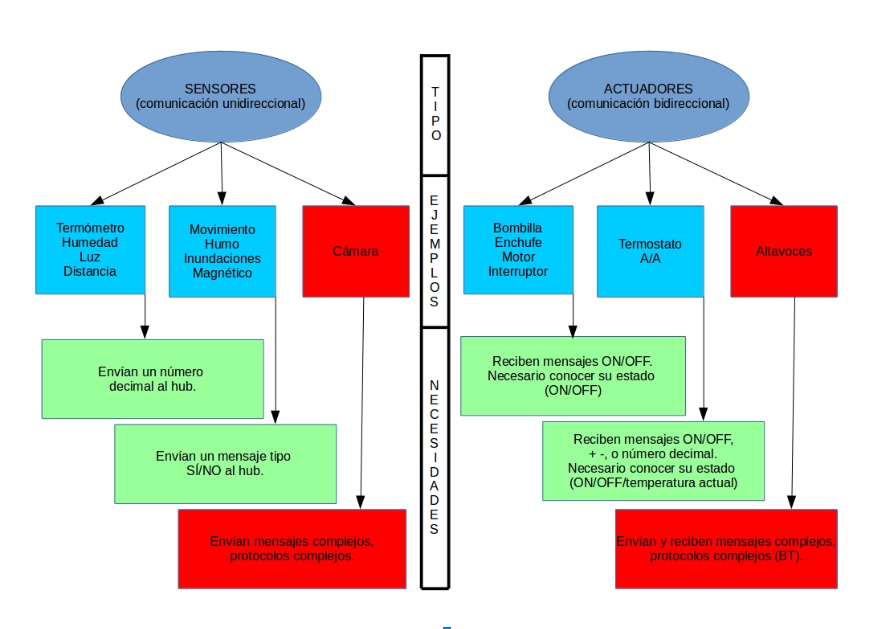
\includegraphics[width=6.00in]{images/descripcion_dispositivos.png}
\caption{Tipos de dispositivos}
\label{fig:descripcion_dispositivos}
\end{figure}


Para la definición del protocolo dividiremos los dispositivos en tres tipos:
\begin{itemize}
\setlength\itemsep{6pt plus 1pt minus 1pt}
\item Tipo 1 (sensores): el hub sólo recibe información de los sensores. El hub no necesita saber qué tipo de información recoge (número decimal, SÍ/NO...etc), simplemente la actualiza y la muestra al usuario.
\item Tipo 2 (actuadores): estos dispositivos envían información al HUB y son capaces de recibir comandos del tipo: ON/OFF, +/-, número decimal...etc.
\item Tipo 3: cámaras IP. Este sensor recibirá un tratamiento especial debido a la necesidad de una comunicación constante y rápida.
\end{itemize}
\subsection{Necesidades del sistema}
Una vez analizadas las necesidades de los dispositivos podemos analizar las necesidades de nuestro sistema.
Para el desarrollo de nuestro sistema necesitaremos una arquitectura que nos permita:
\begin{itemize}
\setlength\itemsep{6pt plus 1pt minus 1pt}
\item \textbf{Comunicación bidireccional entre los dispositivos y el hub:} es necesario que el hub conozca información de los dispositivos, 
registre dispositivos y gestione dispositivos; así como también es necesario que los dispositivos puedan recibir comandos provenientes
del hub.
\item \textbf{Flexibilidad:} el hub debe permitir aceptar dispositivos con diferentes comandos, y no ceñirse sólo a un número cerrado de comandos (ON/OFF, +/-,...).
De esta manera cualquier actuador podrá conectarse al HUB, siempre y cuando los comandos sean registrados de manera correcta.
\item \textbf{Comunicación entre el hub y la interfaz:} será necesario que la información de los dispositivos y el estado de los mismos sea accesible
a través de la interfaz de usuario. Además el usuario debe ser capaz de gestionar los dispositivos y enviar comandos a los actuadores
a través de la interfaz.
\item \textbf{Seguridad en la comunicación:} es imprescindible que toda comunicación se realice de manera segura, de tal manera que nadie pueda modificar o
acceder a nuestra información.
\item \textbf{Escalabilidad:} aunque durante la realización de nuestro proyecto nos centraremos únicamente en la comunicación mediante protocolo HTTPS, 
es necesario diseñar un sistema escalable que el día de mañana pueda funcionar con diferentes protocolos y dispositivos.
\end{itemize}
\lsection{Casos de uso}
Para ayudarnos a diseñar nuestro software, es de gran utilidad un diagrama de casos de uso, en el que se describen
todas las acciones que el usuario puede llevar a cabo.
\par
Además, el diagrama de casos de uso será de gran utilidad a la hora de diseñar la interfaz de nuestra aplicación, ya que para que pueda 
darse un caso de uso es necesario que la interfaz lo contemple.
\subsection{Actores}
Debido a que el usuario podrá interactuar totalmente con el sistema y podrá llevar a cabo acciones irreversibles (como borrar un dispositivo), es necesario
que nuestro sistema cuente con funcinalidad para la gestión de usuarios basada en roles, de tal manera que los usuarios puedan llevar a cabo sólo las acciones
que su rol les permite.
\par
Distinguiremos tres roles de usuario, y por lo tanto, tres actores en nuestro sistema:
\begin{itemize}
\setlength\itemsep{6pt plus 1pt minus 1pt}
\item \textbf{Usuario lurker:} este usuario sólo es capaz de ver el estado actual de los diferentes dispositivos, así como su localización.
\item \textbf{Usuario común:} este usuario, además poder ver el estado y la localización de los dispositivos, puede enviar comandos a los actuadores y gestionar
los dispositivos: eliminarlos, modificar su localización...etc.
\item \textbf{Usuario administrador:} la única diferencia de este usuario con el usuario común es que este usuario es capaz de gestionar usuarios: dar de alta
nuevos usuarios, cambiar el rol de los usuarios y eliminar usuarios.
\end{itemize}
\subsection{Diagrama de casos de uso}

\begin{figure}[H]
\centering
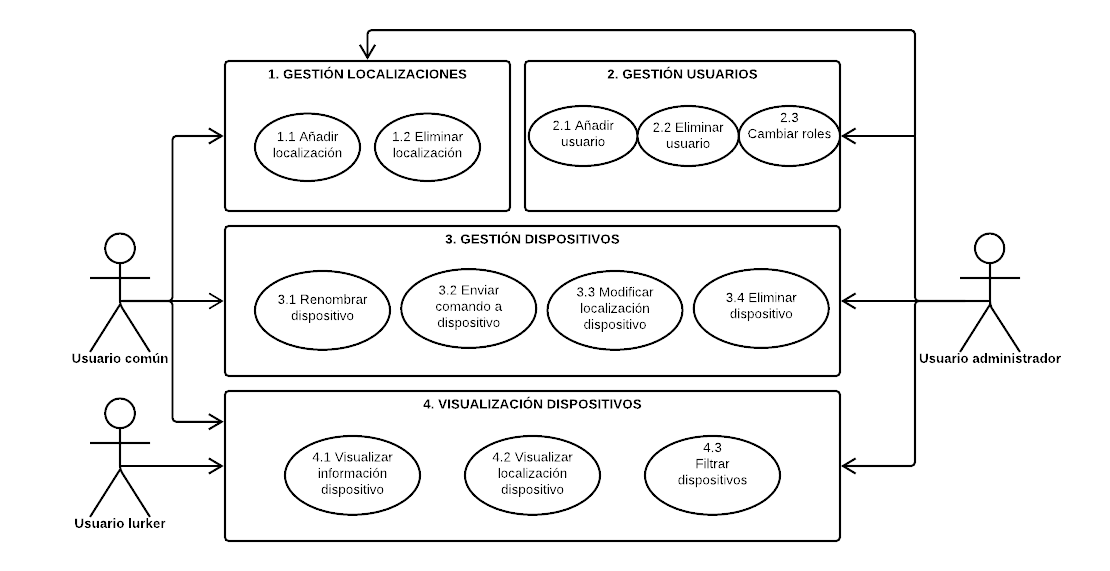
\includegraphics[width=7.00in]{images/casos_uso.png}
\caption{Diagrama de casos de uso}
\label{fig:casos_uso}
\end{figure}

\lsection{Diagramas de secuencia}
Como hemos descrito anteriormente, en nuestro sistema participarán diferentes ``partes`` o subsistemas, por lo que es necesario definir la interacción entre cada
una de ellas. Así como en el diagrama de casos de uso hemos descrito cómo el usuario interactuará con el sistema, en los diagramas de secuencia describiremos
cómo interactuarán nuestros subsistemas entre sí.
\par
Debido a que en la mayoría de casos de uso solamente interactúan el HUB y la interfaz, se realizarán dos diagramas de casos de uso: uno común para todas las acciones
en las que participan HUB e interfaz, y otro con los casos de uso en los que es necesaria la interacción de todos nuestros subsistemas.
\subsection{Subsistemas}
Los subsistemas que participarán en los diagramas de secuencia son:
\begin{itemize}
\item\textbf{HUB}: es la parte central o bridge de nuestro sistema. Se encarga de comunicarse con los dispositivos y con la interfaz de usuario. Única ejecución, contiene también
el servidor de datos.
\item\textbf{Interfaz:} interfaz a través de la cual el usuario podrá interactuar con el HUB y los dispositivos. Se ejecuta en el dispositivo móvil del usuario, por lo 
que existirá una ejecución por cada usuario utilizando la aplicación.
\item\textbf{Dispositivos:} son los encargados de informar al usuario de su estado y, en el caso de los actuadores, ejecutar una acción a partir de un comando.
\end{itemize}
\subsection{Diagrama de secuencia Usuario-Interfaz-Hub}
Este flujo es el que seguirán todos los casos de uso a excepción de los casos \textbf{3.2 Enviar comando a dispositivo} y \textbf{4.1 Visualizar información dispositivo}.
Es el flujo habitual que siguen los frameworks web que utilizan el modelo MVC:
\par
\begin{figure}[H]
\centering
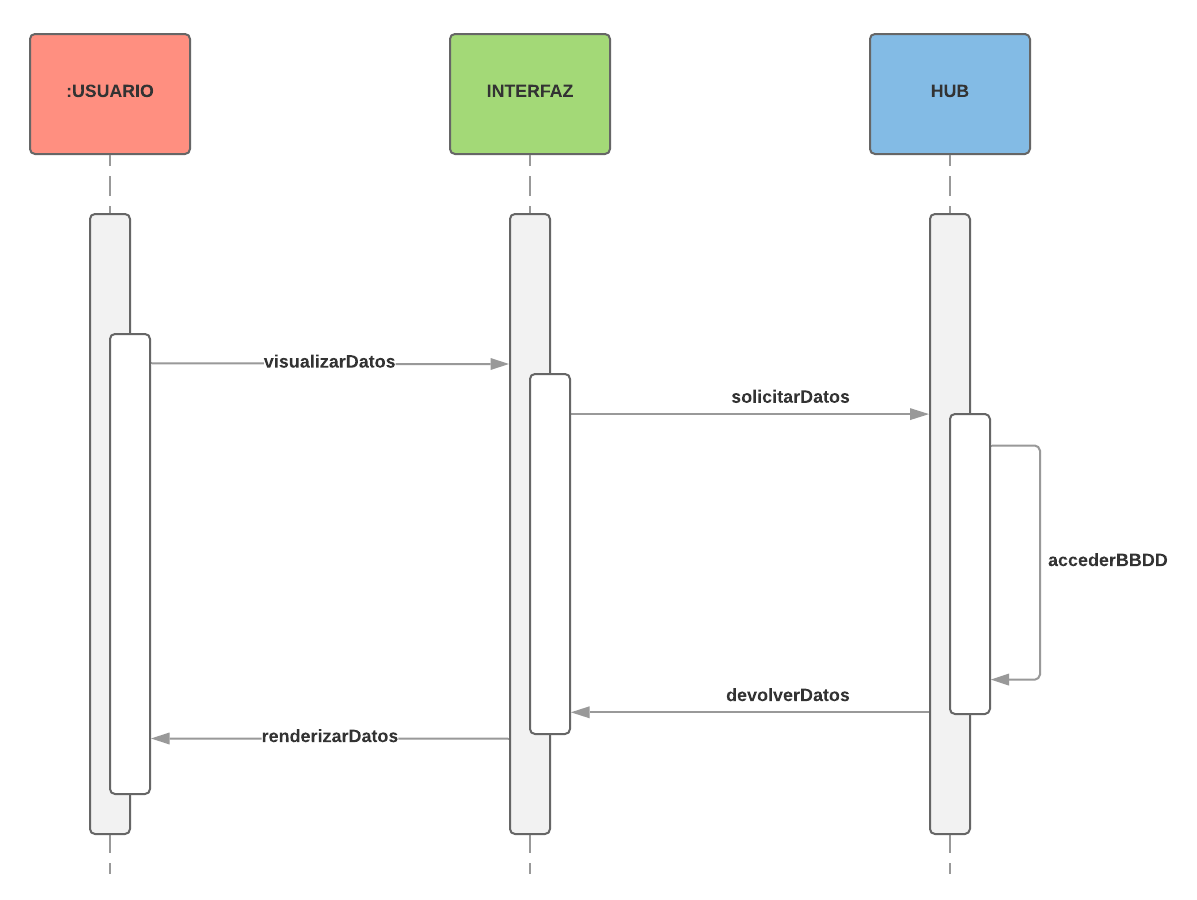
\includegraphics[width=6.00in]{images/diagrama_secuencia_1.png}
\caption{Diagrama de secuencia Usuario-Interfaz-Hub}
\label{fig:diagrama_secuencia_1}
\end{figure}

\subsection{Diagrama secuencia Usuario-Interfaz-Hub-Dispositivos}
En este diagrama se explican dos flujos: 
\begin{itemize}
\item{\textbf{4.1 Visualizar información dispositivo:}} la interfaz, por defecto, muestra la información actualizada de los dispositivos. Los dispositivos mandan su
información al HUB de manera constante, y la interfaz se encarga de pedir el estado de los dispositivos al HUB. 
\item{\textbf{3.2 Enviar comando a dispositivo:}} un usuario desea enviar un comando a un dispositivo. La interfaz envía el comando al HUB, que es el encargado de 
enviárselo al dispositivo.
\end{itemize}
\par
\begin{figure}[H]
\centering
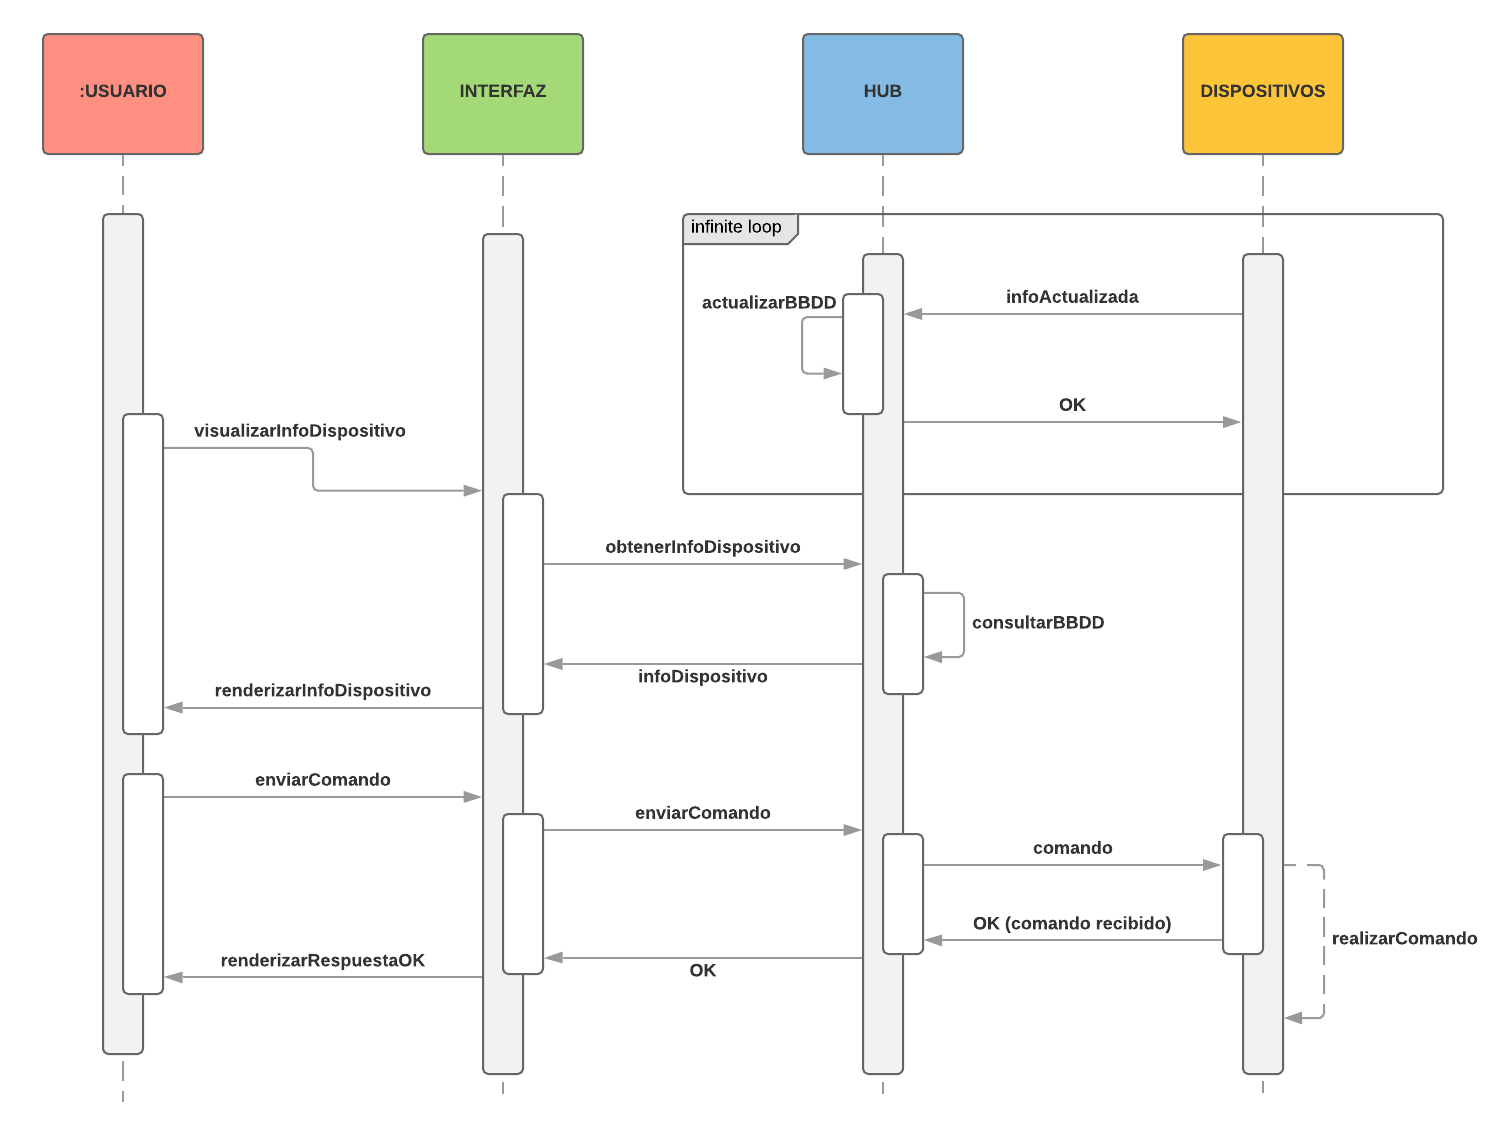
\includegraphics[width=6.00in]{images/diagrama_secuencia_2.png}
\caption{Diagrama de secuencia Usuario-Interfaz-Hub-Dispositivos}
\label{fig:diagrama_secuencia_2}
\end{figure}

\lsection{Protocolo}
En esta sección se describirá el protocolo que se utilizará en las comunicaciones entre los dispositivos y el HUB.
\subsection{Protocolo HTTPS}
El protocolo elegido para la comunicación entre dispositivos, hub e interfaz es el protocolo HTTPS (Hypertext Transfer Protocol Secure).
\par
Este protocolo nos da la posibilidad de implementar una API REST consumible por parte de los dispositivos y por parte de la interfaz,
sin necesidad de utilizar diferentes protocolos en cada caso.
\par
Una API REST proporciona una interfaz entre diferentes sistemas que utilicen HTTP/S como medio comunicación. Las APIs REST están muy estandarizadas a día de hoy y nos dan la capacidad de separar lógica y funcionalidad entre cliente y servidor, y de ser capaces
de utilizar diferentes lenguajes y tecnologías para cada lado. Es decir, podemos tener un servidor escrito en Express.js (JavaScript), una interfaz 
gráfica utilizando Angular5 (TypeScript), y unos actuadores/sensores que utilicen CherryPy (Python).
\par
Además, utilizar HTTPS nos ofrece la posibilidad de crear un canal de comunicación cifrado, de manera que la información que circula en dicho 
canal no pueda ser descifrada por ningún intermediario ni se pueda sufrir un ataque Man-In-The-Middle*.
\lsection{Arquitectura del sistema}
En esta sección se describirá el diseño y la arquitectura del sistema de manera global, incluyendo dispositivos actuadores, 
dispositivos sensores y el propio HUB.
\subsection{Arquitectura del sistema}
Teniendo en cuenta las necesidades de nuestro sistema realizaremos una arquitectura similar a las arquitecturas de microservicios,
en la que el hub y los actuadores serán hosts de un servidor REST y serán capaces de recibir y procesar peticiones.
Esto requerirá n + 1 servidores REST, siendo n el número de dispositivos actuadores.
\par
El hub recibirá peticiones de parte de la interfaz de usuario y de los dispositivos, y lanzará peticiones a los actuadores.
Para ello se establecerán dos APIS que serán publicadas por el HUB y consumidas por la interfaz de usuario y los dispositivos:
\begin{itemize}
\setlength\itemsep{6pt plus 1pt minus 1pt}
\item \underline{Interface API:} será consumida por la interfaz de usuario. Se encargará de enviar la información de los dispositivos al usuario: número
 de dispositivos, información, localización, etc... Además, permitirá al usuario gestionar dispositivos y enviarles comandos.
\item \underline{Sensors API:} será consumida por actuadores y sensores por igual. Permitirá a los dispositivos darse de alta en el sistema y actualizar
periódicamente su información.
\end{itemize}
\par
Los actuadores, además de lanzar peticiones al hub para informar de su estado, deberán ser capaces de recibir peticiones del hub con
diferentes comandos. Para ello se establecerá otra API que todos los dispositivos deberán seguir, para que así el HUB consuma la misma API
en los diferentes dispositivos. Será denominada en adelante como \underline{Actuators API}. Estableceremos y explicaremos estas tres APIs en el capítulo
\textbf{3.3.3 APIS}.
\par
Como mencionamos anteriormente, la seguridad es un requisito indispensable de nuestro sistema, y debemos asegurar que ningún intruso pueda acceder y/o modificar nuestra información.
Para cumplir nuestro requisito, todas las peticiones HTTPS serán securizadas, asegurando así una comunicación segura entre los diferentes servidores.

Esquema de la arquitecura a seguir:
\begin{figure}[H]
\centering
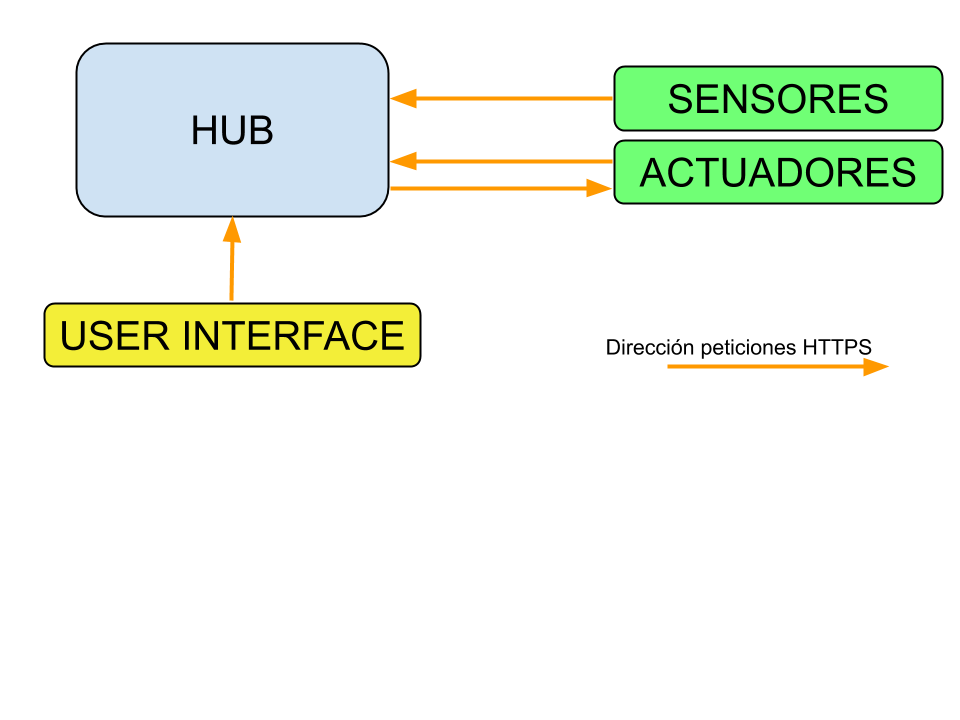
\includegraphics[width=6.00in]{images/esquema_arquitectura.png}
\caption{Esquema de la arquitectura}
\label{fig:esquema_arquitectura}
\end{figure}

\subsection{Modelo de datos}
En esta sección se describirán los modelos de datos a utilizar. Todos los datos residirán en el HUB, que será el encargado de orquestarlos,
organizarlos y mantenerlos.
\par
Analizando las necesidades del sistema nos encontramos con cuatro entidades a definir:
\begin{itemize}
\setlength\itemsep{6pt plus 1pt minus 1pt}
\item \underline{Dispositivos}: esta entidad se utilizará para almacenar la información de los actuadores/sensores. En el caso de los actuadores
será necesario guardar su dirección IP para poder enviarles comandos.
\item \underline{Comandos}: entidad para almacenar los comandos de los diferentes dispositivos. Cada comando tendrá un código y una descripción.
\item \underline{Habitaciones}: esta entidad nace de la necesidad de organizar los dispositivos de una casa en grupos más pequeños. Una manera lógica 
y muy común es por habitaciones, cada dispositivo podrá o no pertenecer a una habitación.
\item \underline{Usuarios}: es necesario restringir los usuarios que pueden tener acceso a nuestro sistema. Las credenciales de cada usuario se guardarán en esta tabla,
así como su rol.
\end{itemize}
Diagrama entidad-relación modelo de datos:
\begin{figure}[H]
\centering
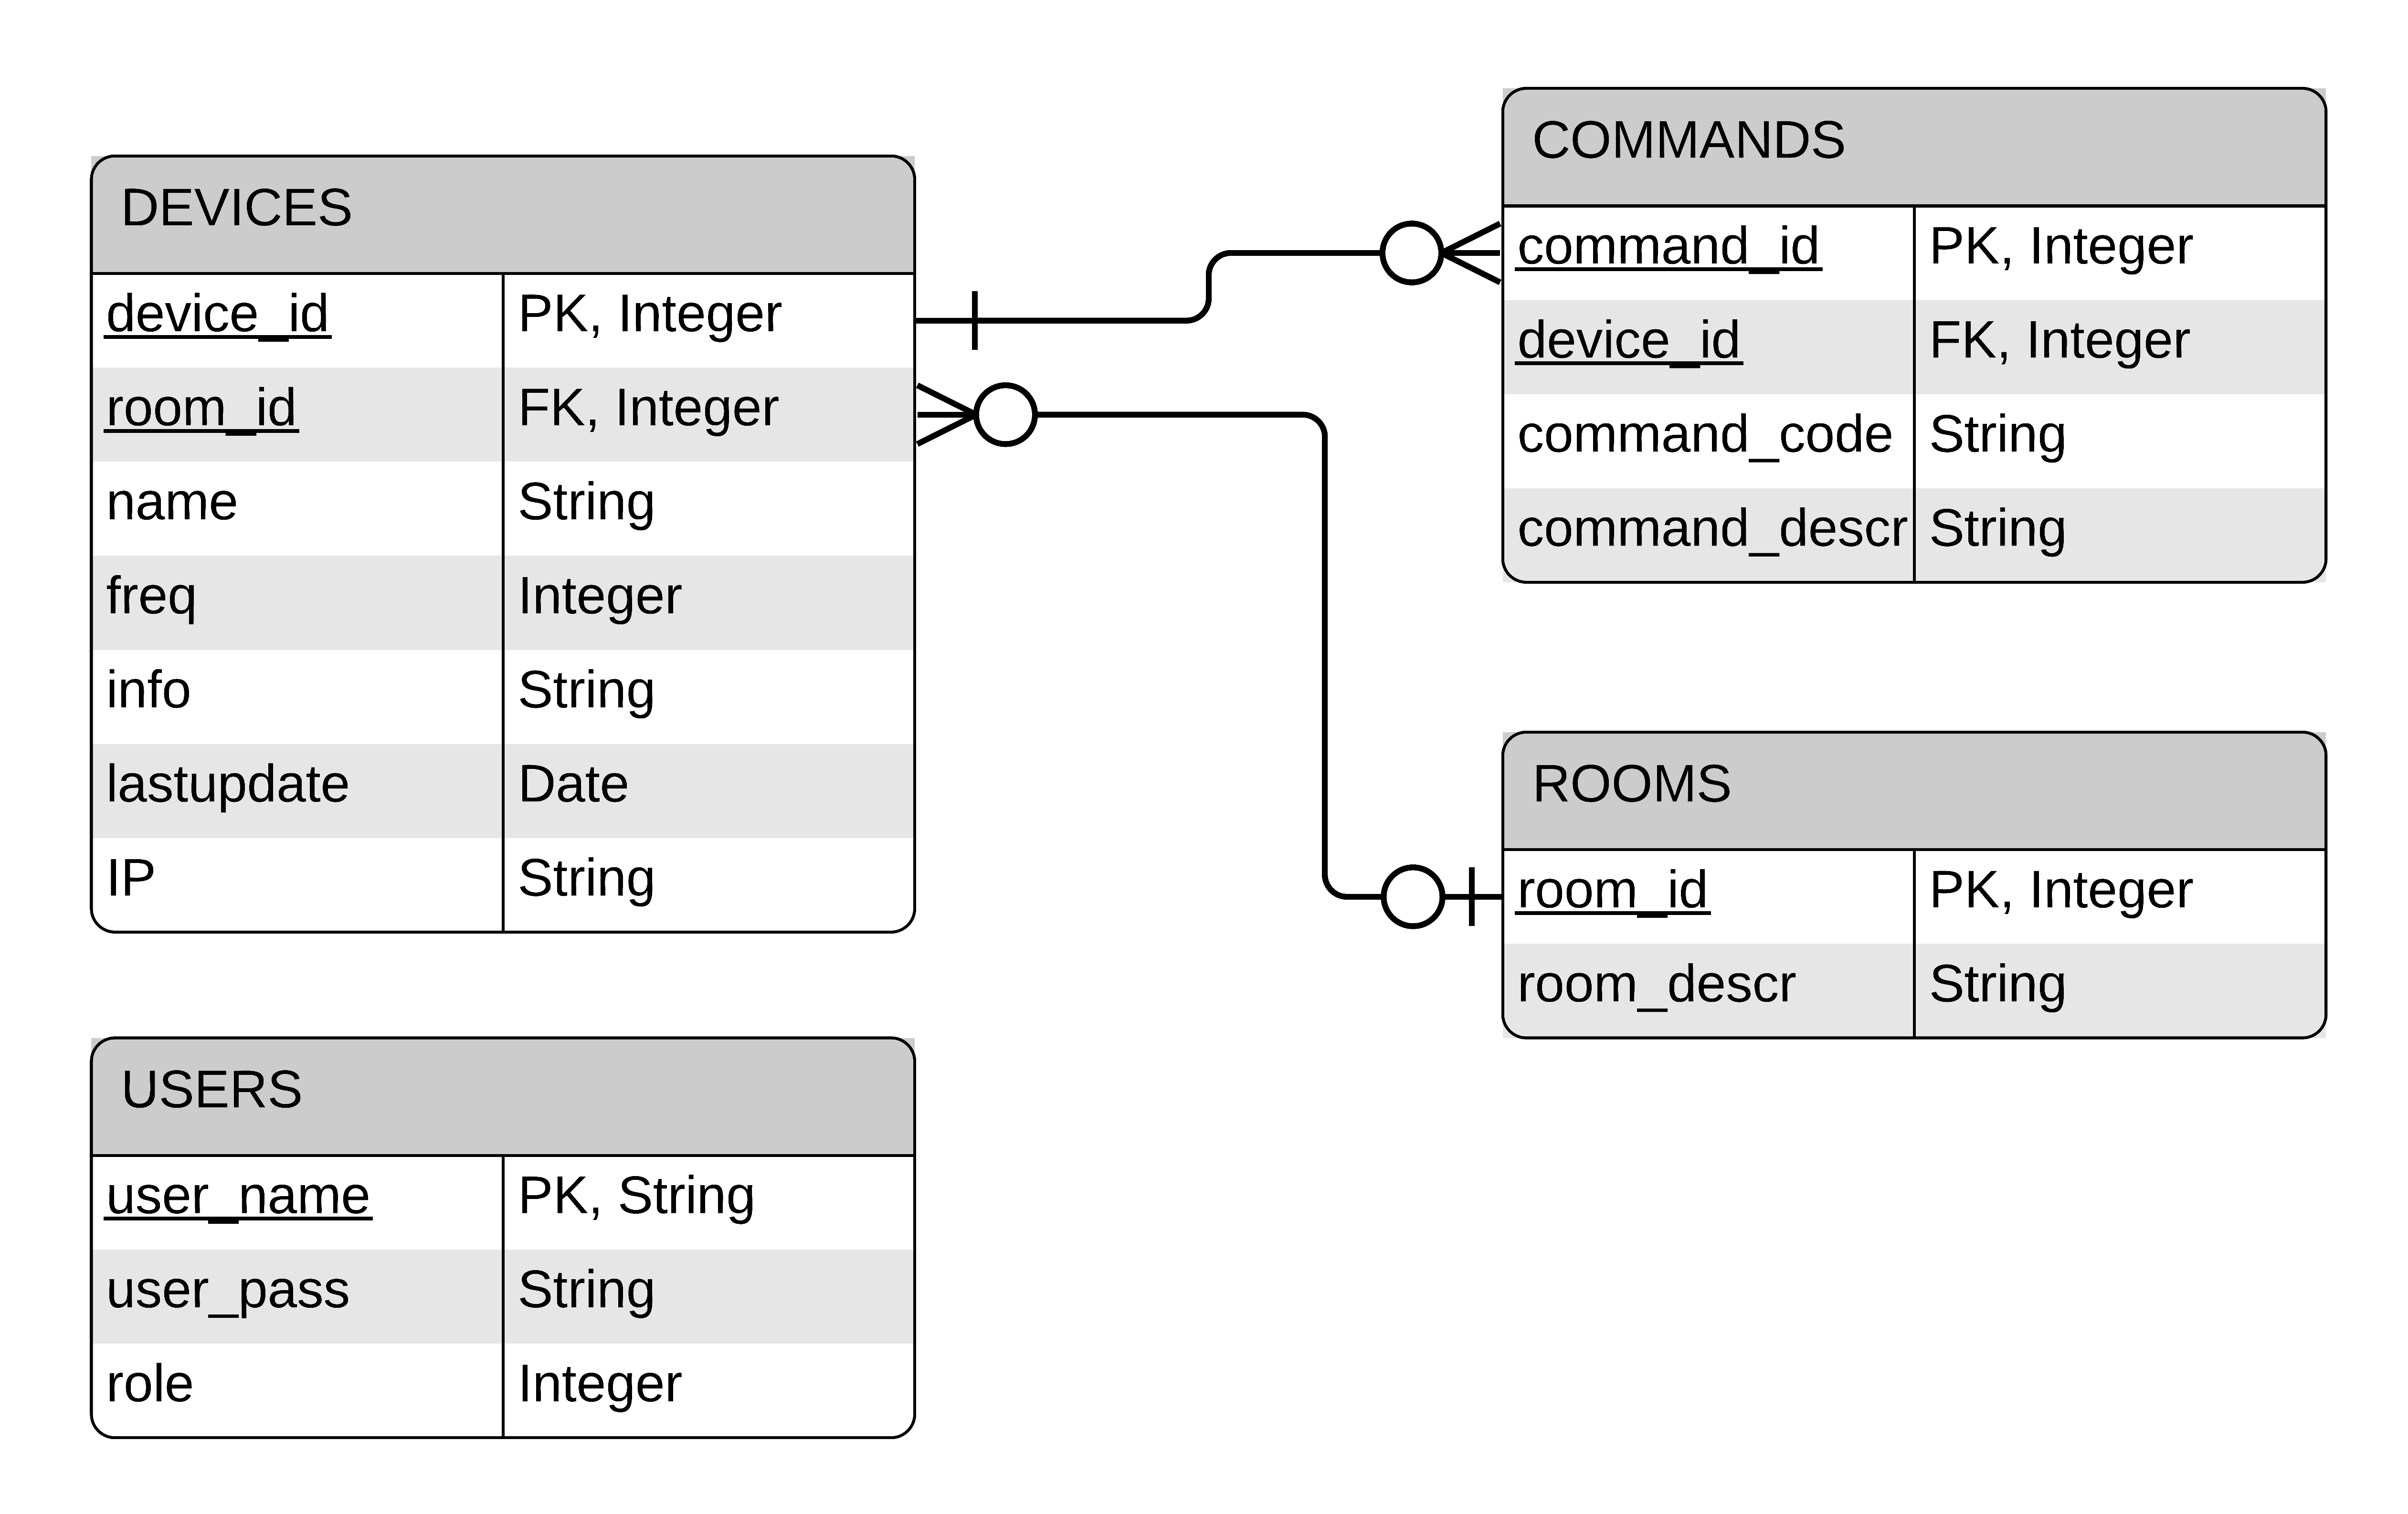
\includegraphics[width=6.00in]{images/er_brimo.png}
\caption{Diagrama ER}
\label{fig:diagrama-er}
\end{figure}
\subsection{APIS}
Una vez numeradas las diferentes APIS a utilizar y definido el modelo de datos podemos comenzar a definir detalladamente cada una de las APIS.
Al tratarse de APIS REST, en la definición
de cada método es necesario informar: ruta del método, verbo (GET, POST, PUT, PATCH, DELETE), cuerpo de la petición (si existiera) y variables
de la ruta (si existieran).
\par
A no ser que se indique lo contrario, el cuerpo de todas las peticiones debe estar en formato JSON, y debe ser
informada la cabecera \textbf{Content-Type} con valor \textbf{application/json}.
\par
Como se ha descrito anteriormente todas las peticiones deberán ir securizadas, para lo que se utilizarán tokens JWT. Es imprescindible que el
token vaya en la cabecera \textbf{x-access-token} de cada petición, o de lo contrario la petición será denegada. La generación de tokens y la gestión
de usuarios es descrita por la API de login.
\par
Estas APIS funcionan como contratos entre publicador y consumidor, y es imprescindible que ambas partes consuman y publiquen de la 
manera acordada para que el sistema completo funcione. El cambio de uno de estos contratos debe ser indicado a todas las partes para que se tenga
en cuenta en los desarrollos futuros.
\par
Todos los métodos de estas APIs están enumerados y definidos en un proyecto de Postman desde el cual se pueden probar.
\par
\subsubsection{Sensors API}
Esta API será consumida tanto por sensores como por actuadores, y les permitirá registrarse en el sistema y actualizar su información.

\begin{itemize}
\setlength\itemsep{6pt plus 1pt minus 1pt}
\item \textbf{POST /brimo/sensors-api/devices}: se utilizará para el registro de dispositivos. En el cuerpo de la petición se informarán
 un nombre descriptivo (podrá ser modificado por el usuario más adelante) y frecuencia
de actualización de la información \footnote{ Si el dispositivo pasa más de los segundos informados sin actualizar información, entonces
el HUB lo considerará desconectado.}. Opcionalmente, en el caso de ser un actuador, el dispositivo informará de los comandos que es capaz
de recibir. Estos comandos vendrán en forma de array y deben contener descripción y código de comando.
Si el registro es correcto el HUB responderá con un 201 CREATED y un id de dispositivo. Este id será utilizado por el dispositivo más adelante
para enviar información al HUB.
\item \textbf{PUT /brimo/sensors-api/devices/\{device-id\}/info}: se utilizará para actualizar la información del dispositivo. El parámetro
device-id indicará el id del dispositivo, proveniente del registro. Si la información se actualiza correctamente el HUB devolverá 200 OK. Una vez
actualizada la información del dispositivo se actualizará la hora de última actualización \textbf{(lastupdate)}.
\end{itemize}

\subsubsection{Actuators API}
Esta API será consumida por el HUB, y permitirá al HUB enviar comandos a los dispositivos.

\begin{itemize}
\setlength\itemsep{6pt plus 1pt minus 1pt}

\item \textbf{POST /brimo/actuators-api/commands?command\_code=ON}: es el único método de la API. El HUB enviará esta petición para enviar
comandos al dispositivo. El código de comando debe haber sido informado previamente en la fase de registro del actuador.

\end{itemize}

\subsubsection{Interface API}
Como hemos explicado anteriormente, esta API será consumida por la interfaz de usuario y permitirá al usuario obtener información de los dispositivos,
gestionarlos y mandarles comandos:

\begin{itemize}
\setlength\itemsep{6pt plus 1pt minus 1pt}
\item \textbf{GET /brimo/interface-api/devices}: esta petición nos devolverá información de todos los dispositivos
dados de alta en el sistema. Al tratarse de una lista no se poblarán todos los campos del dispositivo, sólo los comunes: id del dispositivo, nombre,
frecuencia, fecha de última actualización de la información, id de habitación y descripción de la habitación.
\item \textbf{GET /brimo/interface-api/devices/\{device-id\}}: a diferencia de la petición anterior, se obtiene únicamente la información
del dispositivo indicado con el parámetro device-id. Esta información es más completa, y además de la información de la petición anterior
se obtiene la lista de comandos que acepta el dispositivo y su IP.
\item \textbf{DELETE /brimo/interface-api/devices/\{device-id\}}: a través de esta petición el usuario podrá eliminar el dispositivo indicado. A partir
de este momento el sistema denegará al dispositivo la comunicación con el mismo.
\item \textbf{PATCH /brimo/interface-api/devices/\{device-id\}/?room-id=12\&name=sensor-habitacion}: esta petición permitirá editar la habitación
en la que se encuentra el dispositivo y su nombre. Ambos parámetros room-id y name son opcionales, aunque al menos uno debe estar presente.
\item \textbf{DELETE /brimo/interface-api/devices/\{device-id\}}: a través de esta petición el usuario podrá eliminar el dispositivo indicado. A partir
de este momento el sistema denegará al dispositivo la comunicación con el mismo.
\item \textbf{PATCH /brimo/interface-api/devices/\{device-id\}/?room-id=12\&name=sensor-habitacion}: esta petición permitirá editar la habitación
en la que se encuentra el dispositivo y su nombre. Ambos parámetros room-id y name son opcionales, aunque al menos uno debe estar presente.
\item \textbf{POST /brimo/interface-api/devices/\{device-id\}/commands?command-code=ON}: se utilizará para enviar comandos al dispositivo informado.
La petición irá al HUB, que será el encargado de enviar otra solicitud al dispositivo correspondiente. Para ello, utilizará la IP del dispositivo.
\item \textbf{GET /brimo/interface-api/devices/rooms}: devolverá la lista actual de habtiaciones registradas. Se devolverán en forma de 
array y en cada una de ellas vendrán informadas descripción e identificador.
\item \textbf{POST /brimo/interface-api/devices/rooms}: se utilizará por el usuario para añadir habitaciones. Únicamente es necesario informar
el nombre de la nueva habitación. Si el registro de la habitación es correcto, entonces el HUB devolverá 201 CREATED con el id de la nueva habitación.

\end{itemize}


\subsubsection{Login API}
Esta API será utilizada para la generación de los JWT, que necesariamente, deben ir informados en las cabeceras de cada petición. Además, gestionará
los usuarios con acceso al sistema.
\begin{itemize}
\setlength\itemsep{6pt plus 1pt minus 1pt}
\item \textbf{POST /brimo/login-api}: se deberán informar los campos usuario y contraseña para la correcta generación del token. En el caso
de introducir credenciales inválidas el HUB devolverá 401 Unauthorized. En caso de éxito el HUB devolverá el token generado, que será válido
para las siguientes dos horas.
\item \textbf{POST /brimo/login-api/users}: servirá para añadir nuevos usuarios al sistema. Deberán informarse nombre de usuario y contraseña.
\item \textbf{PUT /brimo/login-api/users}: servirá para modificar la contraseña y/o el nombre de usuario actuales. Deberán ir informados en el
cuerpo de la petición al menos uno de los dos parámetros.
\end{itemize}

\lsection{Diseño de la interfaz gráfica}

Una vez analizados los requisitos de nuestro sistema y diseñado los flujos de datos, podemos pasar a diseñar nuestra interfaz gráfica. Antes de
enumerar las pantallas que tendrá nuestra aplicación y definir el diagrama de actividades, debemos enumerar los requisitos funcionales 

\lsection{Arquitectura del hub}
En esta sección definiremos los módulos que nuestro HUB deberá tener y las funciones que cada uno debe cumplir. La organización por módulos, además
de permitirnos organizar nuestro software de una manera clara, nos ayudará a añadir nuevos módulos y funcionalidad el día de mañana con facilidad.
\par
Por ejemplo, en el módulo de servicios residirá toda la lógica interna, mientras que el módulo enrutador será el encargado de ``traducir`` los datos
provenientes de la red a un modelo de datos conocido e invocar a los diferentes servicios. De esta forma, si en un trabajo futuro queremos añadir
dispositivos bluetooth crearemos un módulo bluetooth que reutilice nuestros servicios.
\par
Otro ejemplo sería la migración de nuestra base de datos a otro motor diferente; sólo necesitaríamos cambiar el módulo repositorio, el resto del sistema
se mantendría intacto.
\par
Cada módulo
debe ser independiente del resto, y la modificación interna de un módulo no debería requerir la modificación del resto de módulos.
\subsection{Módulo enrutador}
Este módulo será el encargado de gestionar las conexiones entrantes y de manejar la información proveniente del exterior. Para nuestro caso, que utilizaremos
el protocolo HTTPS, en este módulo residirán las implementaciones de las APIS anteriormente definidas. Se encargará de implementar todas las rutas, encapsular
los diferentes parámetros en objetos de nuestro modelo y enviar las respuestas y códigos necesarios tras la invocación al módulo de servicios.
\subsection{Módulo middleware}
A pesar de haber separado este módulo del módulo enrutador, este módulo está totalmente ligado a la utilización del protocolo HTTPS. 
Se trata de un módulo totalmente independiente del módulo enrutador, y tendrá dos funciones principales:
\begin{itemize}
\setlength\itemsep{6pt plus 1pt minus 1pt}
\item Interceptar todas las peticiones antes de que lleguen al enrutador y validar las cabeceras y el token JWT. Si el token no es válido entonces
se envía un 401 Unauthorized sin llegar al enrutador.
\item Interceptar los errores que se provoquen durante la ejecución del programa (independientemente del módulo) y traducirlos a respuestas HTTPS. Para esto 
será necesario utilizar un modelo común de error que pueda ser interceptado por este módulo.
\end{itemize}
\subsection{Módulo de servicios}
En este módulo residirá la totalidad de nuestra lógica de negocio. A este módulo ya llegan objetos modelados con nuestro modelo de datos, y es totalmente
independiente del protocolo utilizado. Se encargará de hacer llamadas a los repositorios correspondientes y de aplicar la lógica correspondiente.
\par
Un ejemplo de lógica sería el registro de dispositivos; una vez recibido un dispositivo y sus correspondientes comandos, el servicio se encargará de hacer
las comprobaciones correspondientes y guardar el dispositivo y después sus comandos.
\par
Además, el módulo de servicios transformará los posibles errores provenientes de los repositorios para encapsularlos en errores internos. Un ejemplo sería
transformar un error \textbf{``14 SQLITE\_CANT\_OPEN``} en el siguiente error: \textbf{``Error 01: no se ha podido acceder a la base de datos sqlite``}.
\par
Tanto la entrada como la salida de datos de los métodos de nuestros servicios seguirán el modelo de datos del HUB.
\subsection{Módulo repositorio}
Este módulo contendrá toda la gestión de los datos del HUB. Será invocado por el módulo de servicios, y 
será el encargado de gestionar las conexiones con la base de datos e insertar/obtener datos de la misma.
Este módulo recibe datos modelados con nuestro modelo de datos, pero no necesariamente la manera de enviarlos/guardarlos tiene que coincidir con nuestro modelo 
de datos. Sin embargo, el retorno de los métodos de este módulo si serán datos modelados.
\par
Si en un futuro se realizasen llamadas a terceros, una API de Google por ejemplo, las llamadas a esas APIS también se realizarían desde este módulo.
\subsection{Vista general}
Por lo tanto, el diseño esquemático de la arquitectura interna del hub sería el siguiente:
\begin{figure}[H]
\centering
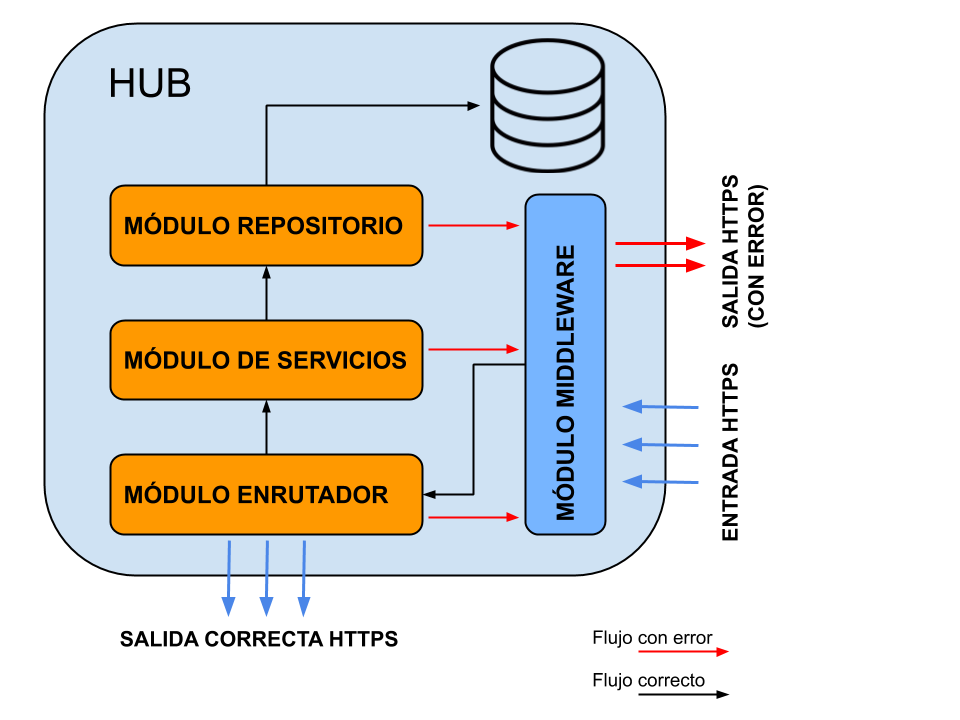
\includegraphics[width=6.00in]{images/arquitectura_hub.png}
\caption{Arquitectura interna del hub}
\label{fig:arquitectura_hub}
\end{figure}
